%\documentclass[handout]{beamer}
\documentclass[compress]{beamer}

%\documentclass{beamer}
\usepackage[T1]{fontenc}
\usepackage{pifont}
\usepackage{threeparttable}
\usepackage{subcaption}
\usepackage{tikz-qtree}
\usepackage{listings}
\usepackage[american]{babel}
\usepackage{csquotes}
\usepackage[style=apa, backend=biber]{biblatex}
\usepackage{tikz}
\usepackage{multicol}
\usepackage{booktabs}
\usepackage{graphicx}
\usepackage{neuralnetwork}
\usepackage{hyperref}

\usepackage{minted}
\definecolor{listingbg}{rgb}{0.87,0.93,1}
\setminted[python]{
breaklines,
linenos,
fontsize=\scriptsize,
frame=single,
xleftmargin=0pt}

\hypersetup{
    pdfborder={0 0 0},
    colorlinks=true,
}
\usetheme[block=fill,subsectionpage=progressbar,sectionpage=progressbar]{metropolis} 

\definecolor{Purple}{HTML}{911146}
\definecolor{Orange}{HTML}{CF4A30}

\setbeamercolor{alerted text}{fg=Orange}
\setbeamercolor{frametitle}{bg=Purple}

\setbeamercovered{still covered={\opaqueness<1->{5}},again covered={\opaqueness<1->{100}}}

\lstset{
    basicstyle=\scriptsize\ttfamily,
    columns=flexible,
    breaklines=true,
    numbers=left,
    %stepsize=1,
    numberstyle=\tiny,
    backgroundcolor=\color[rgb]{0.85,0.90,1}
}

\lstnewenvironment{lstlistingoutput}{\lstset{
        basicstyle=\footnotesize\ttfamily,
        columns=flexible,
        breaklines=true,
        numbers=left,
        %stepsize=1,
        numberstyle=\tiny,
        backgroundcolor=\color[rgb]{.7,.7,.7}}}{}


\lstnewenvironment{lstlistingoutputtiny}{\lstset{
        basicstyle=\tiny\ttfamily,
        columns=flexible,
        breaklines=true,
        numbers=left,
        %stepsize=1,
        numberstyle=\tiny,
        backgroundcolor=\color[rgb]{.7,.7,.7}}}{}

\renewcommand*{\bibfont}{\tiny}

\makeatletter
\setbeamertemplate{headline}{%
    \begin{beamercolorbox}[colsep=1.5pt]{upper separation line head}
    \end{beamercolorbox}
    \begin{beamercolorbox}{section in head/foot}
        \vskip2pt\insertnavigation{\paperwidth}\vskip2pt
    \end{beamercolorbox}%
    \begin{beamercolorbox}[colsep=1.5pt]{lower separation line head}
    \end{beamercolorbox}
}
\makeatother

\newcommand{\question}[1]{
    \begin{frame}[plain]
        \begin{columns}
            \column{.4\textwidth}
            \makebox[\columnwidth]{
                
\includegraphics[width=\columnwidth,height=\paperheight,keepaspectratio]{../pictures/mannetje.png}}
            \column{.6\textwidth}
            \large
            \textcolor{orange}{\textbf{\emph{#1}}}
        \end{columns}
    \end{frame}}

\newcommand{\instruction}[1]{\emph{\textcolor{gray}{[#1]}}}

\addbibresource{../resources/literature.bib}
\graphicspath{{../resources/pictures/}}

\title[Computational Communication Science 2]{\textbf{Computational Communication Science 2} \\Week 6 - Lecture\\ »Setting Up Supervised Machine Learning«}
\author[A. Marthe Möller]{Marthe Möller \\ ~ \\ \footnotesize{a.m.moller@uva.nl} \\}
\date{May 8, 2023}
\institute[Digital Society Minor, University of Amsterdam]{Digital Society Minor, University of Amsterdam}

\begin{document}
	
\begin{frame}{}
	\titlepage
\end{frame}
	
\begin{frame}{Today}
	\begin{tiny}
	\tableofcontents
	\end{tiny}
\end{frame}


\section{Recap}

\begin{frame}[fragile]{What we did so far}
Week 1 - 3: Text as data \\\
Week 4: Recommender systems \\\

Use Python to set up an experiment (research project)!
\end{frame}

\begin{frame}[fragile]{What we will do next}
Week 6 - 7: Automated analysis of text with Supervised Machine Learning \\\

Use Python to analyze texts - and reflect on this!
\end{frame}


\begin{frame}[fragile]{What we will do next} 
	
Classical content analysis:	
Manual analysis of texts
\end{frame}

\begin{frame}[fragile]{What we will do next} 
	
This can be done automatically with Python!
	
Especially helpful when working with big data sets.
\end{frame}


\section{Rule-based Text Classification}

\begin{frame}[fragile]{Text classification}

Text classification: To assign a label to a text.

\pause
\normalsize

\begin{alertblock}{For example, to distinguish between:}
	\begin{itemize}
	\item newspaper articles about sports vs. economics.
	\item reliable vs. unreliable information about vaccination.
	\item webpages about holding companies vs. financing companies.
	\item positive vs. negative movie reviews.
\end{itemize}
\end{alertblock}
\end{frame}


\begin{frame}[fragile]{Text classification}
	
RQ: How prevalent is flaming on Twitter?
	
\pause
\normalsize
	
\begin{alertblock}{Rule-based approach:}
	\begin{itemize}
	\item Create a list with all the swearwords that exist.
	\item For each tweet in the dataset, use the list to count the number of swearwords	
	\item If a tweet contains X number of swearwords label it as flaming
	\end{itemize}
\end{alertblock}
\end{frame}


\begin{frame}[fragile]{Sentiment Analysis}

We can add nuance by creating more rules.

\pause

For example, in sentiment analyses, we can include a rule telling the machine what to do in case of negation or modifiers.

"This movie is really not good." \\
"This movie is really good." 

\pause

When you simply want to count the occurence of specific words, a rule-based approach will be quick, cheap, easy, and transparent - perfect!

\end{frame}


\begin{frame}[fragile]{Text classification}
	
\begin{alertblock}{Advantages of rule-based text classification:}
	\begin{itemize}
		\item Simple and therefore transparant
		\item Cheap
	\end{itemize}

\end{alertblock}
\end{frame}


\begin{frame}[fragile]{Text classification}
	
\begin{alertblock}{Challenges of rule-based text classification:}
	\begin{itemize}
	\item Not a suitable way to anayze latent or abstract variables 
	\pause
	\item You must know all the categories beforehand
	\pause
	\item You must know and be able to express all the rules
	\end{itemize}

% what are examples of latent variables for which rule-based approaches may not work?
\end{alertblock}
\end{frame}


\begin{frame}{From Rule-based to Automated}
	
When it is easy for humans to decide to what class a text belongs, but we struggle to translate our decision process into straight-forward rules, we are likely to be better of using a form of automated text classification: Supervised Machine Learning.
	
\end{frame}


\begin{frame}{What is SML?}
	
\begin{center}
	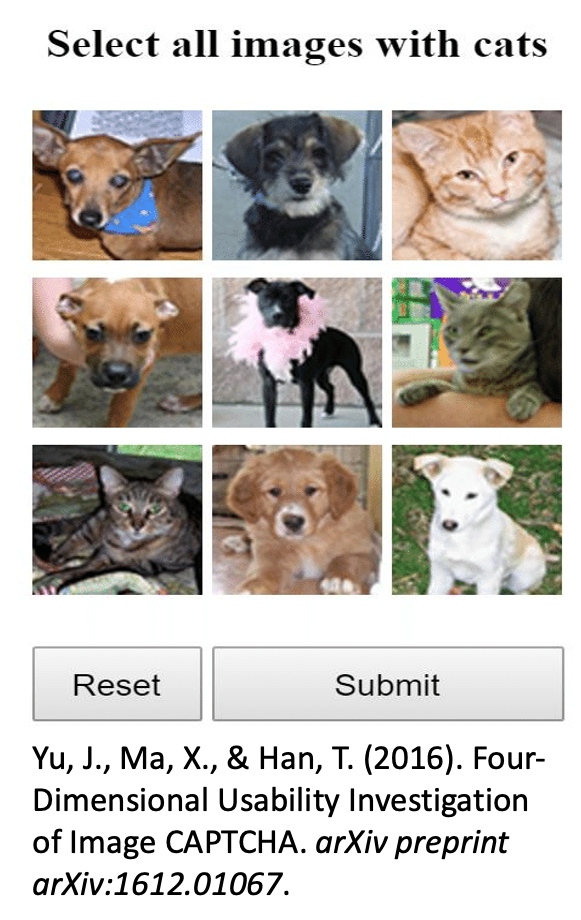
\includegraphics[width=4cm, height=7cm]{../pictures/CAPTCHA.png} 
\end{center}
\end{frame}


\begin{frame}{What is SML?}
	
\begin{center}
	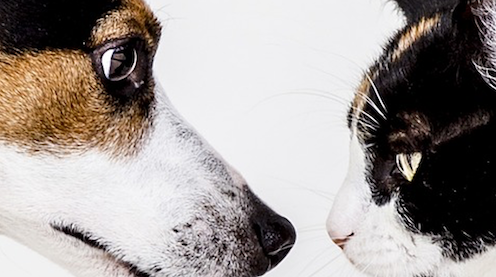
\includegraphics{../pictures/dogvscat.png}
\end{center}
	
\begin{tiny}
	Read more about this project in: 
	\fullcite{sermanet_overfeat_2014} 
\end{tiny}
\end{frame}



\begin{frame}{What is ML?} 
	
Machine Learning: “a type of artificial intelligence in which computers use huge amounts of data to learn how to do tasks rather than being programmed to do them.” \\\
	
\begin{tiny}
	Oxford Dictionary
\end{tiny}
	
\end{frame}

\begin{frame}{What is SML?} 
	
Supervised Machine Learning (SML): “A form of machine learning, where we aim to predict a variable that, for a least part of our data is known.” \\\
	
\begin{tiny}
	\fullcite{van_atteveldt_computational_2022} 
\end{tiny}
\end{frame}


\begin{frame}{What is SML?} 

“The goal of Supervised Machine Learning: estimate a model based on some data, and then use the model to predict the expected outcome for some new cases, for which we do not know the outcome yet.” \\\
	
\begin{tiny}
	\fullcite{van_atteveldt_computational_2022} 
\end{tiny}
\end{frame}


\begin{frame}[fragile]{What is SML?} 
Machine Learning has a lot of similarities to regression analysis!
\end{frame}



\begin{frame}[fragile]{Zooming out} 
	
\begin{alertblock}{We talked about:}
\begin{itemize}
	\item Rule-based Text Classification
	\item Automated Text Classification: SML
\end{itemize}
\end{alertblock}
	
\begin{alertblock}{Next, we will talk about:}
\begin{itemize}
	\item The principles behind SML
	\item Some commonly used SML models
\end{itemize}
\end{alertblock}	
\end{frame}


\section{The principles behind SML}

\begin{frame}[fragile]{The principles behind SML} 
	
\(y = constant + b_1 * x_1 + b_2 * x_2\) 

\pause

\(y\) = Is this a dog? ( 0 = definitely no, 1 = definitely yes)
\pause
\(x_1\) = bark? (0= no, 1 = yes) \\\
\pause
\(x_2\) = tail? (0 = no, 1 = yes) \\\
	
\end{frame}

\begin{frame}[fragile]{The principles behind SML} 
	
\(y = constant + b_1 * x_1 + b_2 * x_2\)
\pause
	
\(y = 0 + 0.8 * x_1 + 0.2 * x_2\) 
\end{frame}


\begin{frame}[fragile]{The principles behind SML} 
	
\(y = 0 + 0.8 * 1 + 0.2 * 0\)
\pause
	
\(0.8 = 0 + 0.8 * 1 + 0.2 * 0\)
\end{frame}


\begin{frame}{The principles behind SML} 
	
\(0.8 = 0 + 0.8 * 1 + 0.2 * 0\)\\\

\pause
	
Classification: a predictive modeling problem where a class label is predicted for a given example of input data. 
\end{frame}


\begin{frame}{The principles behind SML}
	
\begin{center}
	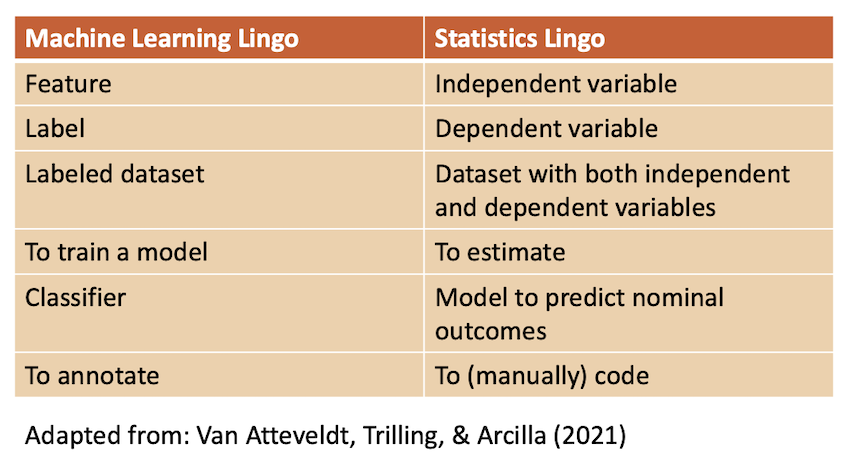
\includegraphics[width=\linewidth,height=\textheight,keepaspectratio]{../pictures/MLlingo.png} \\\
\end{center}	
\end{frame}


\begin{frame}[fragile]{The principles behind SML} 
	
Traditional usage of models in CS: to explain \\\
\pause

Usage of models in ML: to predict \\\
\end{frame}

\begin{frame}{The principles behind SML} 
	
Compare: \\\
	
RQ: To what extent does the amount of hours spend playing violent video games predict aggressive behavior by individuals? \\\
	
RQ: Given the amount of hours that an individual spents playing violen video games, how likely is this person to show aggressive behavior?
	
\end{frame}


\begin{frame}{The principles behind SML} 
	
Can you think of an example case where SML can be useful?
	
\end{frame}


\begin{frame}{The principles behind SML} 
You know know about the principles of SML. \\\
	
What does the process of SML look like?
\end{frame}


\begin{frame}{SML step by step}
	
\begin{center}
	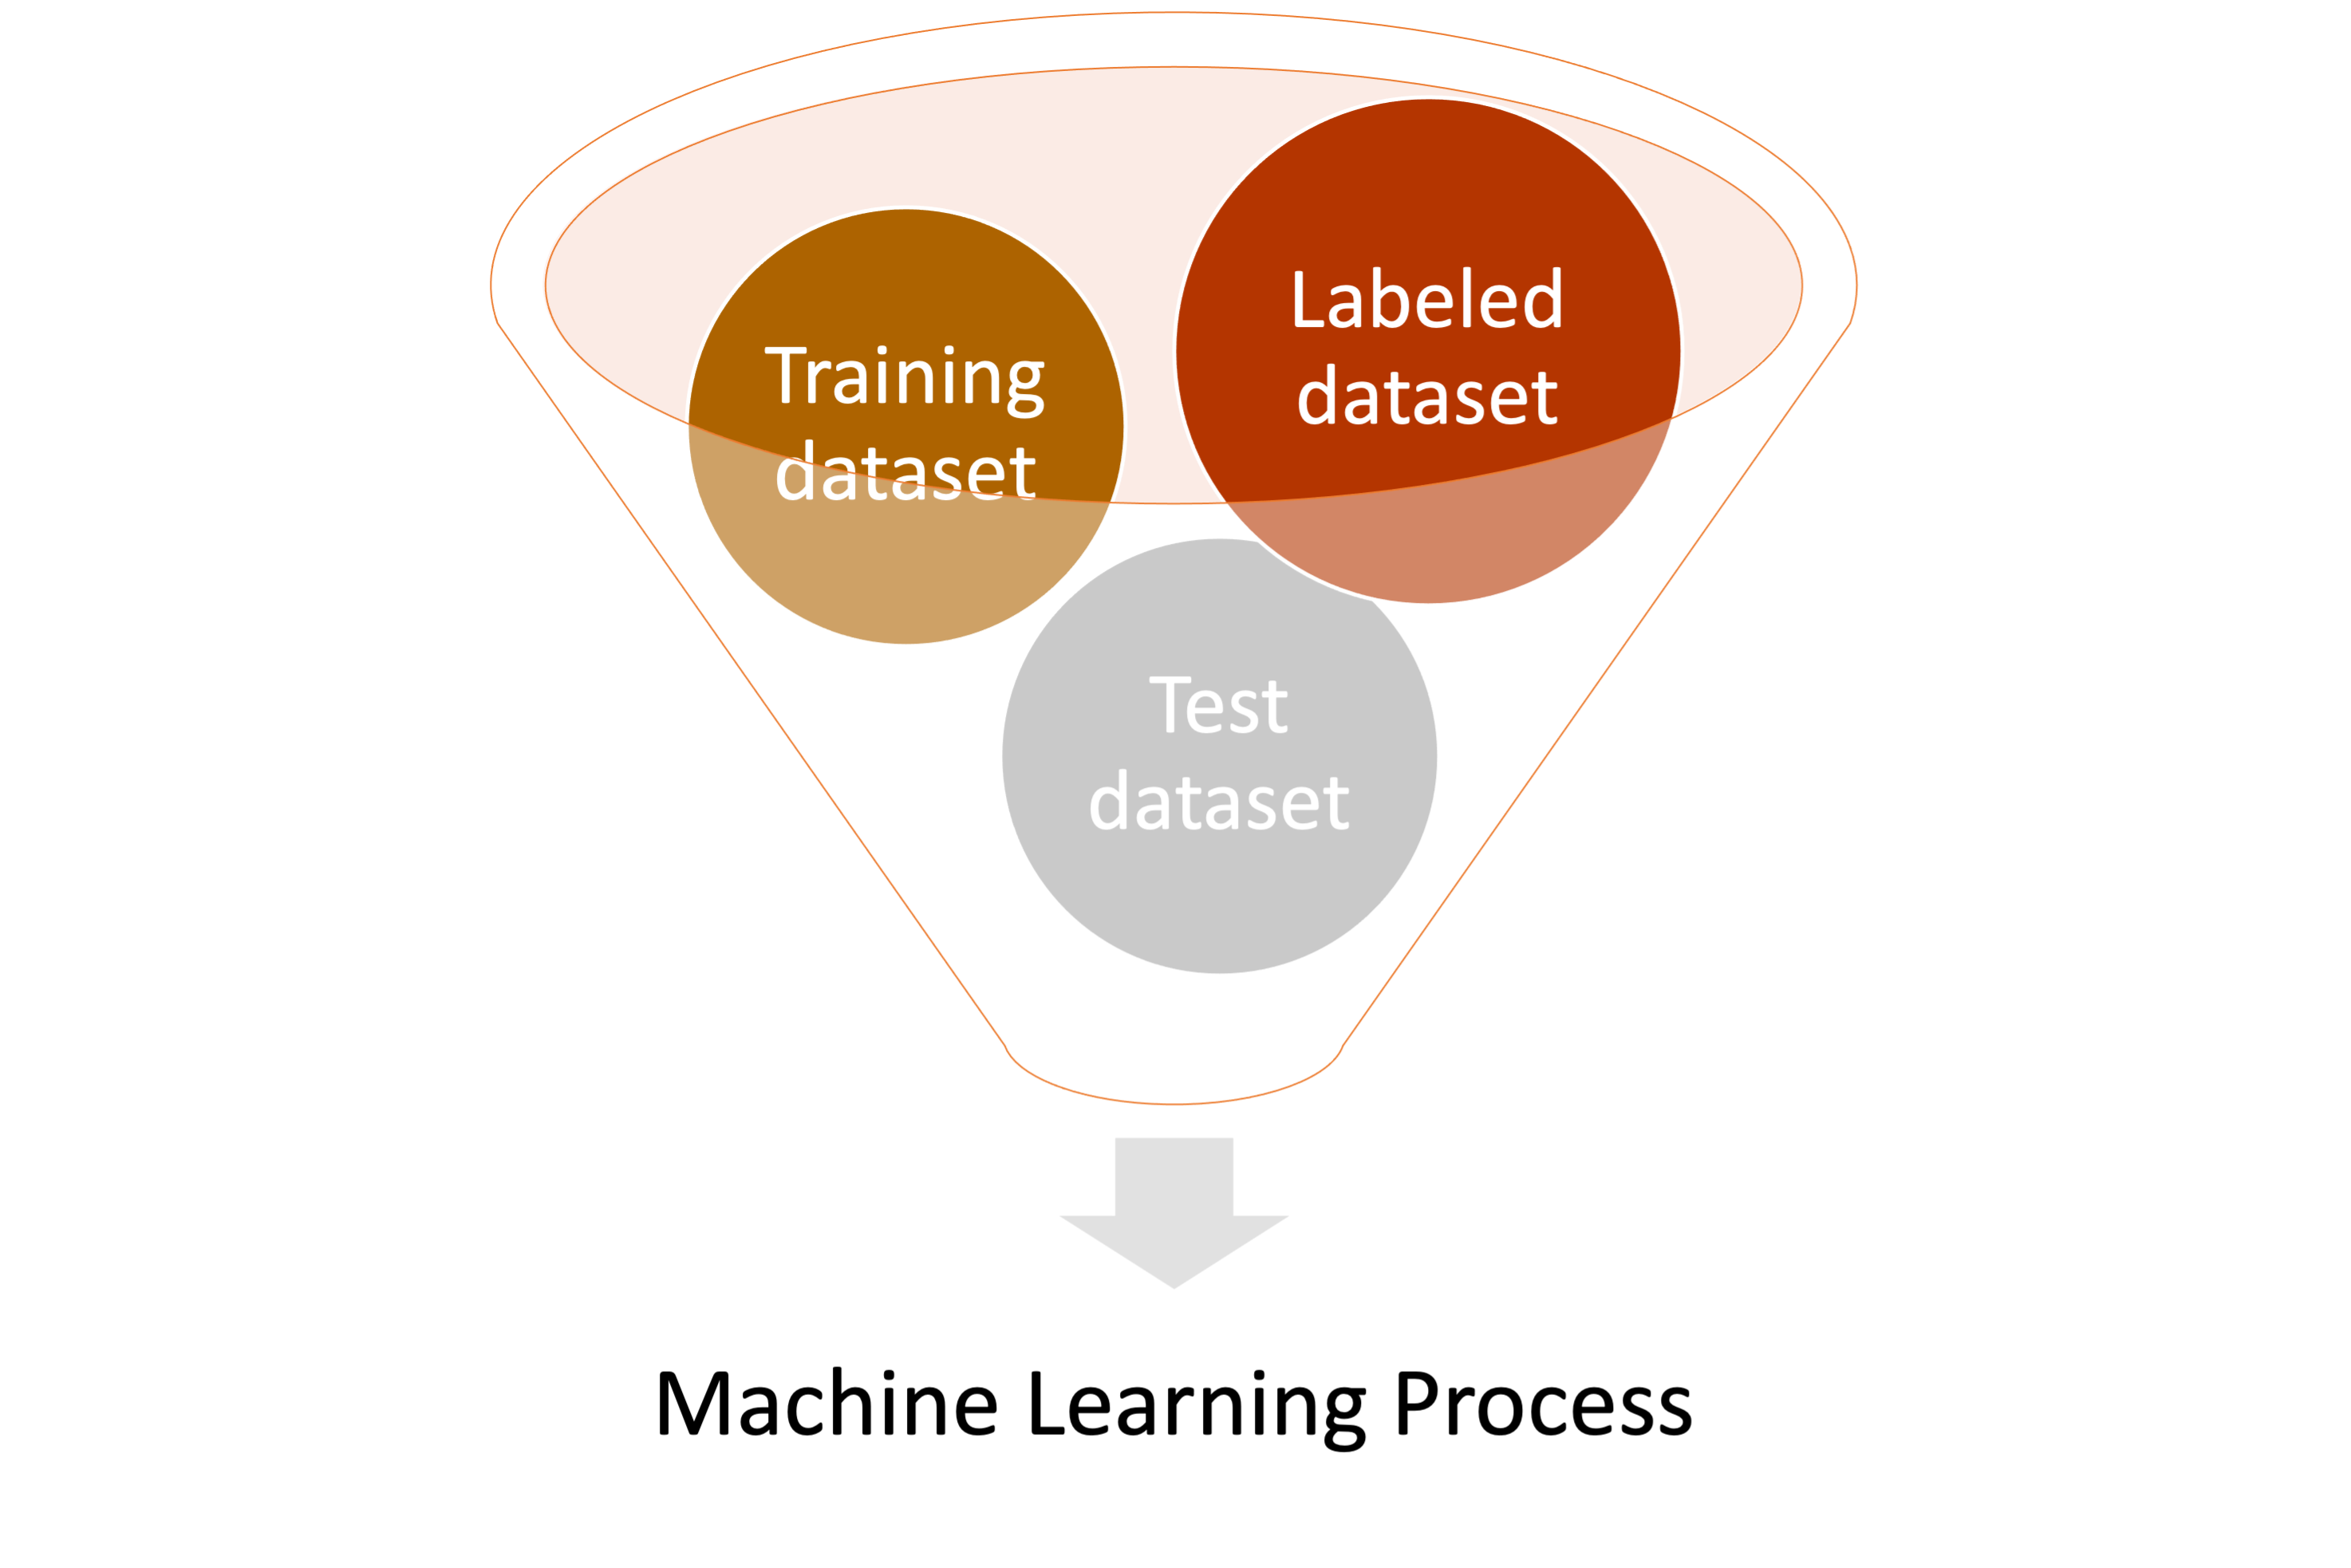
\includegraphics[width=\linewidth,height=\textheight,keepaspectratio]{../pictures/MLingredients.png} \\\
\end{center}
\end{frame}


\begin{frame}{SML step by step}
	
\begin{center}
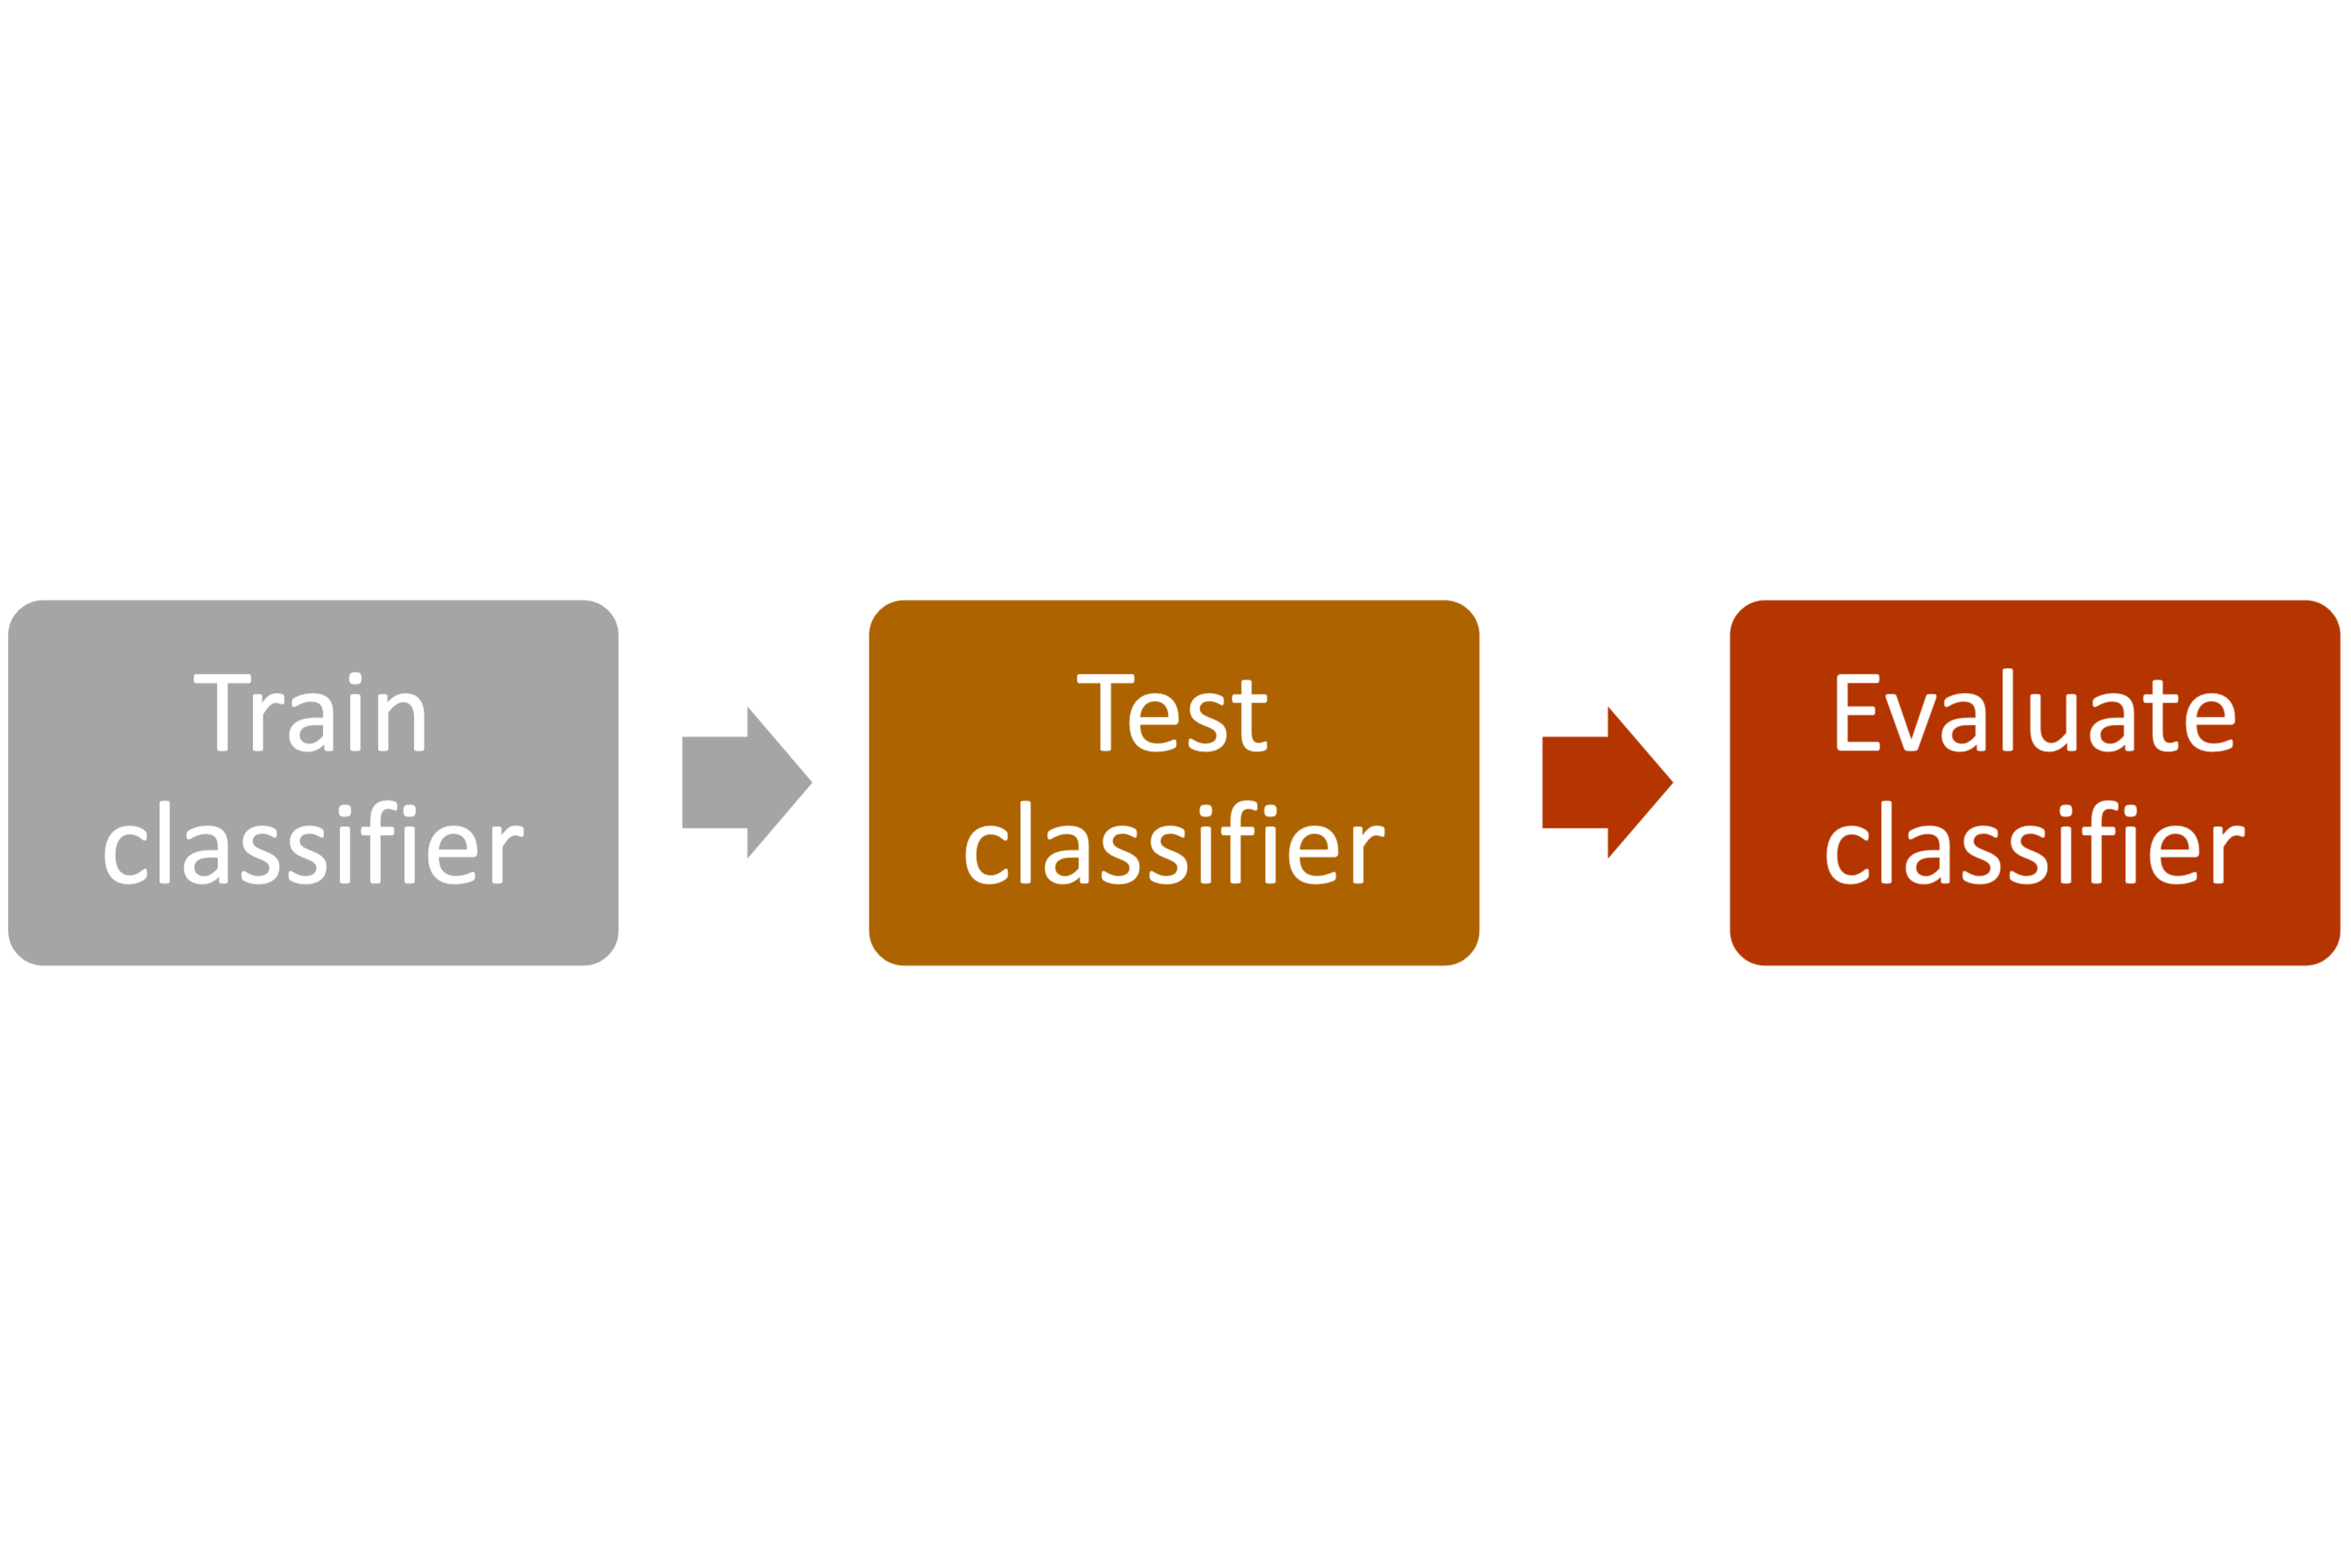
\includegraphics[width=\linewidth,height=\textheight,keepaspectratio]{../pictures/MLprocess.png} \\\
\end{center}
\end{frame}


\begin{frame}{SML step by step}
	
Today, more about the first step! \\\

(Next week, more about the second and last step)
\end{frame}


\begin{frame}[fragile]{Zooming out} 
	
\begin{alertblock}{We talked about:}
	\begin{itemize}
		\item Rule-based Text Classification
		\item Automated Text Classification: SML
		\item The principles behind SML
	\end{itemize}
\end{alertblock}
	
\begin{alertblock}{Next, we will talk about:}
	\begin{itemize}
		\item A practical application of SML
		\item Some commonly used SML models
	\end{itemize}
\end{alertblock}	
	
\end{frame}


\section{SML: A practical application}

\begin{frame}{Regression}
	
\begin{center}
	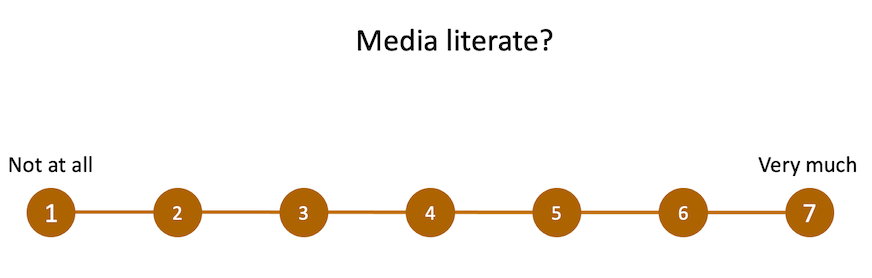
\includegraphics[width=\linewidth,height=\textheight,keepaspectratio]{../pictures/medialiteracyscale.png} \\\
\end{center}
	
\end{frame}


\begin{frame}{Logistic Regression}
	
\begin{center}
	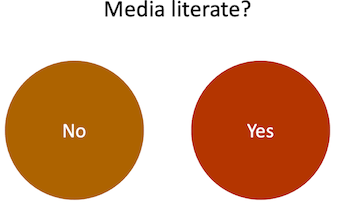
\includegraphics{../pictures/medialiteracydummy.png} \\\
\end{center}
\end{frame}


\begin{frame}{Logistic Regression}
	
\begin{center}
	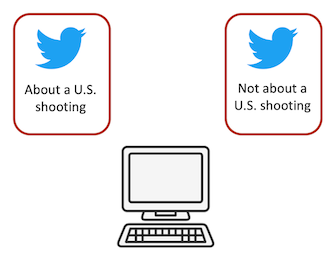
\includegraphics{../pictures/Zhangetal_1.png} \\\
\end{center}
	
\begin{tiny}
	\fullcite{zhang_whose_2019} 
\end{tiny}
\end{frame}


\begin{frame}{Logistic Regression}
	
\begin{center}
	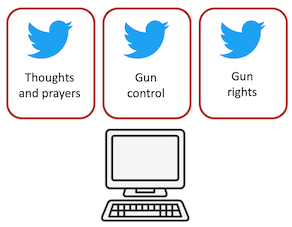
\includegraphics{../pictures/Zhangetal_2.png} \\\
\end{center}
	
\begin{tiny}
	\fullcite{zhang_whose_2019} 
\end{tiny}
		
\end{frame}


\begin{frame}{Logistic Regression}
	
\begin{center}
	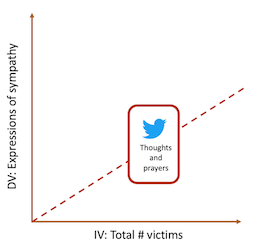
\includegraphics{../pictures/Zhangetal_3.png} \\\
\end{center}
	
\begin{tiny}
	\fullcite{zhang_whose_2019} 
\end{tiny}	
\end{frame}


\begin{frame}[fragile]{What does this look like in code?}
	
First, we need to read in the ingredients we need for SML: 
	
\begin{lstlisting}
import csv
from sklearn.model_selection import train_test_split

tweets = []
labels = []

with open(file) as fi:
  data = csv.reader(fi, delimiter='\t')
  for row in data:
    tweets.append(row[0])
    labels.append(row[1])

tweets_train, tweets_test, y_train, y_test = train_test_split(tweets, labels, test_size=0.2, random_state=42)
\end{lstlisting}
\end{frame}


\begin{frame}[fragile]{What does this look like in code?}
	
Four lists: 
	
\begin{lstlistingoutput}

tweets_train = ['Tweet about shooting', 'Another tweet', 'Shooting!']
tweets_test = ['One more tweet']

y_train = [1, 0, 1]	
y_test = [0]	

\end{lstlistingoutput}
\end{frame}



\begin{frame}[fragile]{What does this look like in code?}
	
Second, vectorize the texts that need to be labeled: 
	
\begin{lstlisting}
from sklearn.feature_extraction.text import (TfidfVectorizer)
		
tfidfvectorizer = TfidfVectorizer(stop_words="english")
X_train = tfidfvectorizer.fit_transform(tweets_train)
X_test = tfidfvectorizer.transform(tweets_test)
		
\end{lstlisting}
	
Where tweets\_train and tweets\_test are two lists with tweets (strings)
	
\end{frame}


\begin{frame}[fragile]{What does this look like in code?}
	
Next, I train my machine and test it: 
	
\begin{lstlisting}
from sklearn.linear_model import (LogisticRegression)
		
logres = LogisticRegression()
logres.fit(X_train, labels_train)
y_pred = logres.predict(X_test)
\end{lstlisting}
\end{frame}


\begin{frame}[fragile]{What does this look like in code?}
	
To train a model based on a tf-idf vectorizer and Log Regression:
	
\begin{lstlisting}
from sklearn.feature_extraction.text import (TfidfVectorizer)
from sklearn.linear_model import (LogisticRegression)
		
tfidfvectorizer = TfidfVectorizer(stop_words="english")
X_train = tfidfvectorizer.fit_transform(tweets_train)
X_test = tfidfvectorizer.transform(tweets_test)
		
logres = LogisticRegression()
logres.fit(X_train, labels_train)
y_pred = logres.predict(X_test)
\end{lstlisting}
	
\end{frame}


\begin{frame}[fragile]{SML models}
	
Logistic Regression is one commonly used model to train classifiers. \\\
Let's talk about other models as well!
	
\end{frame}


\section{SML models}

\begin{frame}{Na\"{\i}ve Bayes}
	
\begin{center}
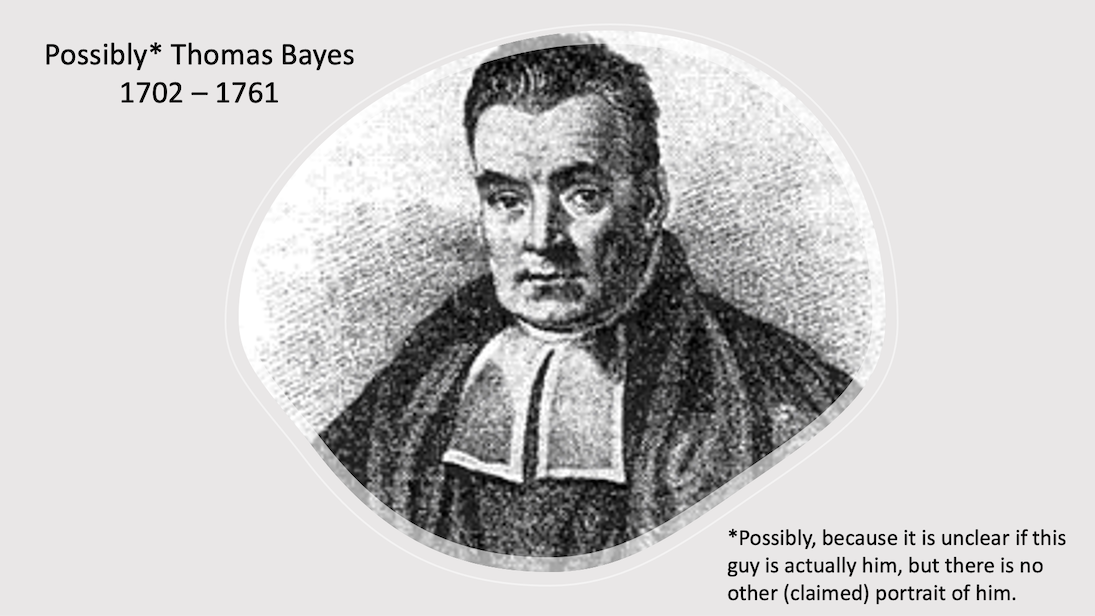
\includegraphics[width=\linewidth,height=\textheight,keepaspectratio]{../pictures/ThomasBayes.png} \\\
\end{center}
\end{frame}



\begin{frame}{Na\"{\i}ve Bayes}
	
$ P(\rm{A} \mid \rm{B}) = \frac{P(\rm{B} \mid \rm{A}) \cdot P(\rm{A})}{P(\rm{B})} $
	
Mathematicians’ language for: the probability of A if B is the case/present/true. 
	
$ P(\rm{label} \mid \rm{features}) = \frac{P(\rm{features} \mid \rm{label}) \cdot P(\rm{label})}{P(\rm{features})} $

\end{frame}



\begin{frame}[fragile]{What does this look like in code?}
	
Let's also train a model based on a count vectorizer and Naïve Bayes:
	
\begin{lstlisting}
from sklearn.feature_extraction.text import (CountVectorizer)
from sklearn.naive_bayes import MultinomialNBB
		
countvectorizer = CountVectorizer(stop_words="english")
X_train = countvectorizer.fit_transform(texts_train)
X_test = countvectorizer.transform(texts_test)
		
nb = MultinomialNB()
nb.fit(X_train, labels_train)
y_pred = nb.predict(X_test)
\end{lstlisting}
	
\end{frame}


\begin{frame}{Support Vector Machines}
	
SVMs aim to find a hyperplane in an \(N\)-dimensional space that distinctly classifies the datapoints. 
	
The best hyperplane is the one that has the maximum margin (distance) between the datapoints of both classes.
	
\begin{center}
	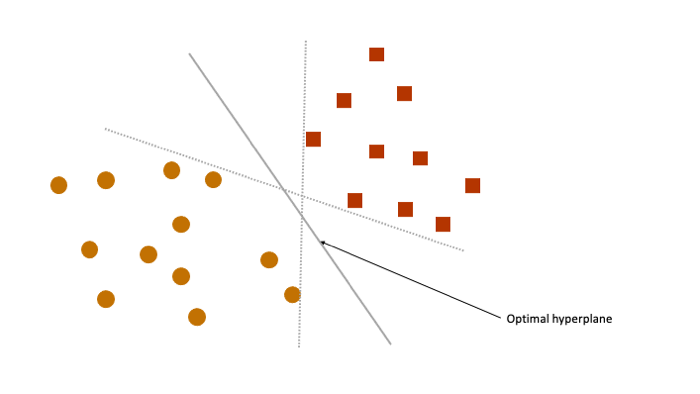
\includegraphics[width=\linewidth,height=0.5\textheight,keepaspectratio]{../pictures/optimal_hyperplane.png} \\\
\end{center}
	
\end{frame}


\begin{frame}{Support Vector Machines}
	
\begin{center}
	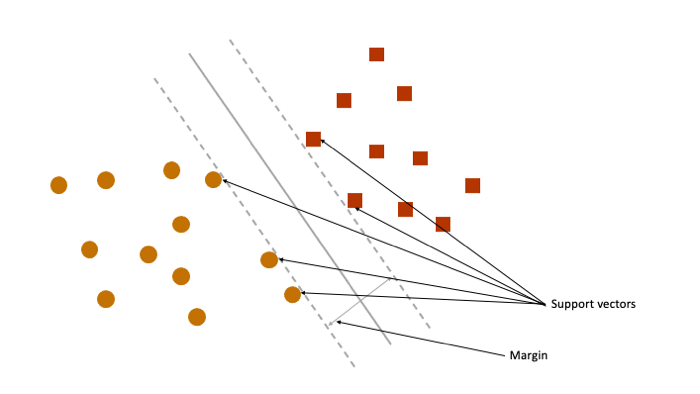
\includegraphics[width=\linewidth,height=\textheight,keepaspectratio]{../pictures/SVM.png} \\\
\end{center}
\end{frame}


\begin{frame}{Decision Trees and Random Forests}
	
\begin{center}
	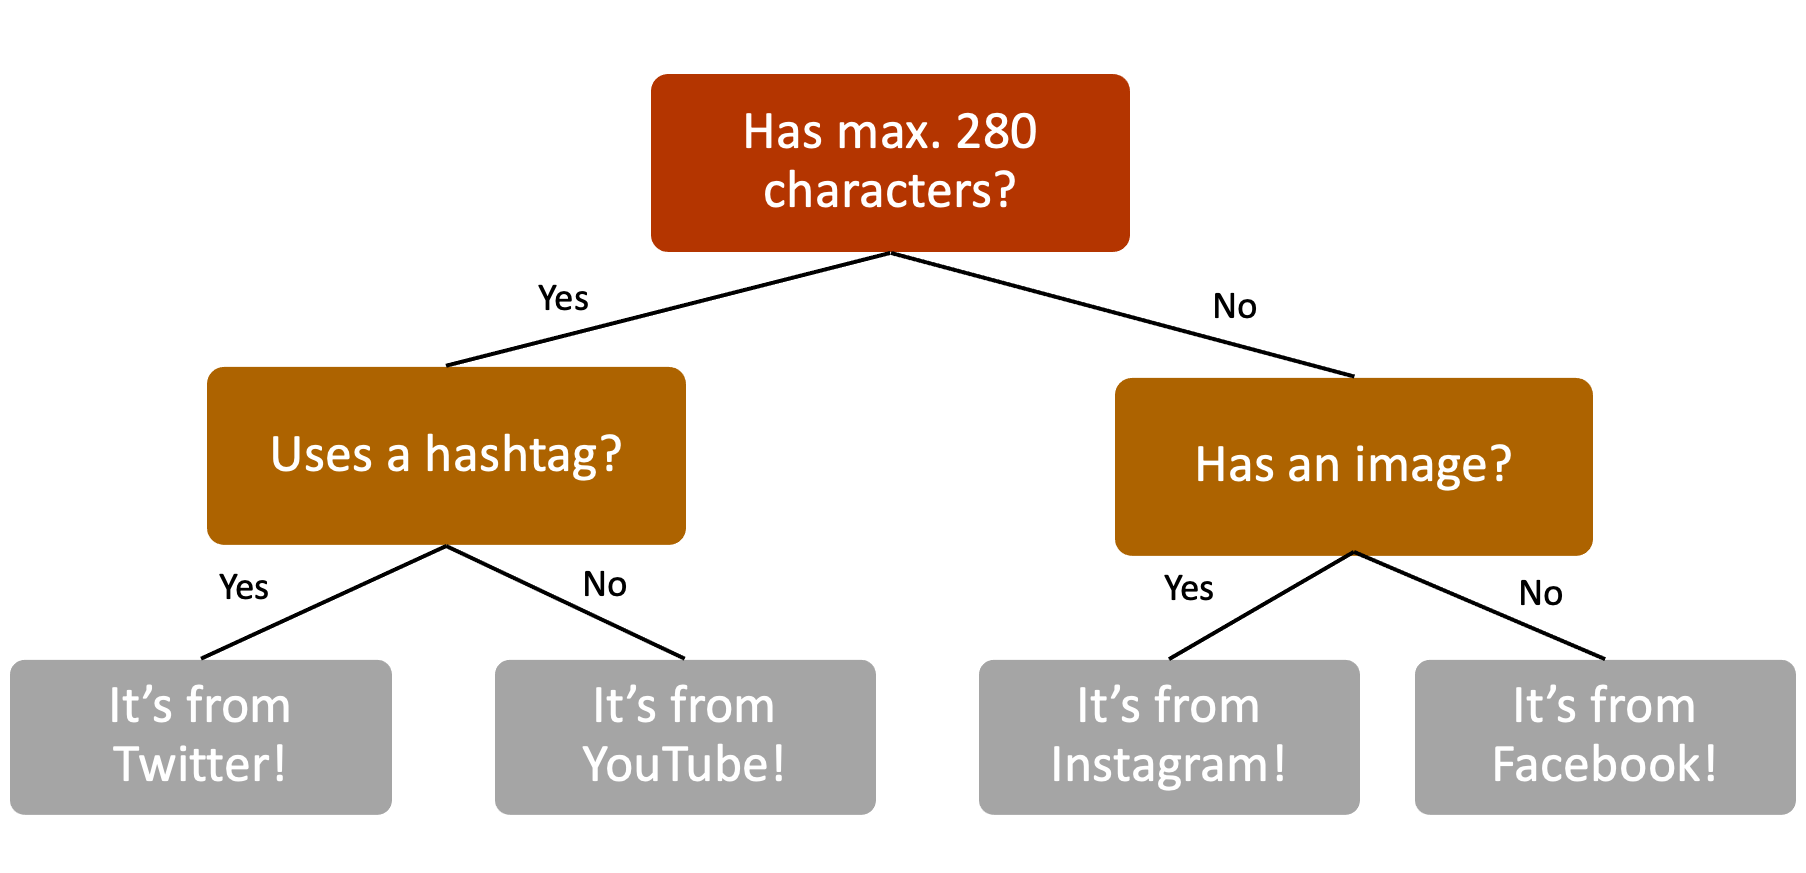
\includegraphics[width=\linewidth,height=\textheight,keepaspectratio]{../pictures/decisiontree.png} \\\
\end{center}
\end{frame}



\begin{frame}[fragile]{Decision Trees and Random Forests} 
	
	\begin{alertblock}{Advantages of decision trees:}
		\begin{itemize}
			\item Transparency
			\item  Suitable for non-linear relationships
		\end{itemize}
	\end{alertblock}
	
	\begin{alertblock}{Disadvatanges of decision trees:}
		\begin{itemize}
			\item Loss of nuance due to yes/no-design
			\item Cannot correct early mistakes
			\item Prone to overfitting
		\end{itemize}
	\end{alertblock}	
	
\end{frame}


\begin{frame}{Decision Trees and Random Forests}
	
\begin{center}
	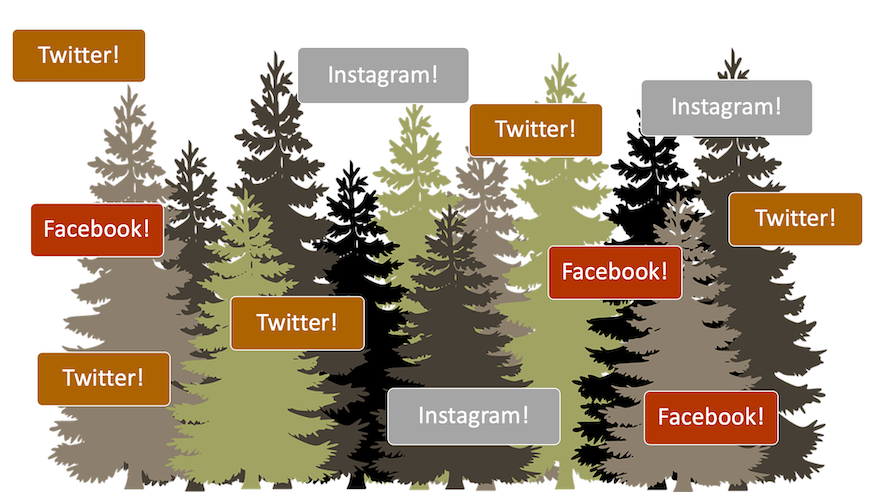
\includegraphics[width=\linewidth,height=\textheight,keepaspectratio]{../pictures/randomforest.png} \\\
\end{center}
\end{frame}


\begin{frame}{Recap}
	
Many different models available for machine learning.
	
How do you know what is the best for your case? Try it out and validate!
	
\end{frame}


\begin{frame}[fragile]{Zooming out} 
	
	\begin{alertblock}{Today, we talked about:}
		\begin{itemize}
			\item Rule-based Text Classification
			\item Automated Text Classification: SML
			\item The principles behind SML
			\item A practical application of SML
			\item Some commonly used ML models
		\end{itemize}
	\end{alertblock}
\end{frame}



\begin{frame}[fragile]{Zooming out} 
	
\begin{alertblock}{Tomorrow and this week, you will:}
	\begin{itemize}
		\item Get some hands-on experience with supervised machine learning!
	\end{itemize}
\end{alertblock}

Work on the the tutorial exercises for this week. \\\
\end{frame}

\begin{frame}
	\frametitle{Refs}
	\printbibliography
\end{frame}
	

\end{document}